%%%%%%%%%%%%%%%%%%%%%%%%%%%%%%%%%%%%%%%%%%%%%%%%%%%%%%%%%%%%%%%%%%%%%%%%%%%%%%%%%%%%%%%%%%%%%%
%%%%%%%%%%%%%%%%%%%%%%%%%%%%%%%%%%%%%%%%%%%%%%%%%%%%%%%%%%%%%%%%%%%%%%%%%%%%%%%%%%%%%%%%%%%%%%
%%%%%%%%%%% GPU
%%%%%%%%%%%%%%%%%%%%%%%%%%%%%%%%%%%%%%%%%%%%%%%%%%%%%%%%%%%%%%%%%%%%%%%%%%%%%%%%%%%%%%%%%%%%%%
%%%%%%%%%%%%%%%%%%%%%%%%%%%%%%%%%%%%%%%%%%%%%%%%%%%%%%%%%%%%%%%%%%%%%%%%%%%%%%%%%%%%%%%%%%%%%%

% \cleardoublepage
\chapter{Equalizer Equations}
\label{chap:eq_eq}

\section{Overview}
This thesis examines that performance and GPU implementation of 5 equalizers.
While the performance and GPU implementation is interesting, this thesis makes no claim of theoretically expanding understanding of equalizers.
The data-aided equalizers studied in this thesis are:
\begin{itemize}
\item Zero-Forcing (ZF)
\item Minimum Mean Square Error (MMSE)
\item Constant Modulus Algorithm (CMA)
\item Frequency Domain Equalizer 1 (FDE1)
\item Frequency Domain Equalizer 2 (FDE2)
\end{itemize}

The ZF and MMSE equalizers are very similar in formulation though from different sources.
As you might tell from the names, FDE1 and FDE2 are very similar also with one subtle difference.
CMA isn't related to any other algorithm aside from being initialized to MMSE.

\section{Zero-Forcing and Minimum Mean Square Error Equalizers}

The ZF and MMSE equalizers are treated together here because they have many common features.
Both equalizers are found by solving linear equations
\begin{equation}
\mathbf{R}\mathbf{c} = \hat{\mathbf{h}}
\end{equation}
where $\mathbf{c}$ is vector of the desired equalizer coefficients
and $\mathbf{R}$ is the auto-correlation matrix of the channel estimate $\hat{\mathbf{h}}$.
It will be shown that the only difference between ZF and MMSE lies in the the auto-correlation matrix $\mathbf{R}$.

\subsection{Zero-Forcing}
The ZF equalizer is an FIR filter defined by the coefficients
\begin{equation}
\begin{matrix}
c_\text{ZF}(-L_1) & \cdots & c_\text{ZF}(0) & \cdots & c_\text{ZF}(L_2).
\end{matrix}
\end{equation}
The filter coefficients are the solution to the matrix vector equation \cite[eq. (311)]{PAQ-phase1}
\begin{equation}
\mathbf{c}_\text{ZF} = \big(\mathbf{H}^\dagger\mathbf{H}\big)^{-1} \mathbf{H}^\dagger \mathbf{u}_{n_0}
\label{eq:c_ZF_direct}
\end{equation}
where
\begin{equation}
\mathbf{c}_\text{ZF} = 
\begin{bmatrix}
c_\text{ZF}(-L_1) \\ \vdots \\ c_\text{ZF}(0) \\ \vdots \\ c_\text{ZF}(L_2)
\end{bmatrix},
\end{equation}
\begin{equation}
\mathbf{u}_{n_0} = \begin{bmatrix} 0 \\ \vdots \\ 0 \\ 1 \\ 0 \\ \vdots \\ 0 \end{bmatrix}
	\begin{matrix*}[l] \left. \vphantom{\begin{matrix} 0 \\ \vdots \\ 0 \end{matrix}} \right\}
		\text{$n_0-1$ zeros}
		\\ \\
		\left. \vphantom{\begin{matrix} 0 \\ \vdots \\ 0 \end{matrix}} \right\}
		\text{$N_1+N_2+L_1+L_2-n_0+1$ zeros}
		\end{matrix*},
		\label{eq:un0_ZF}
\end{equation}
and
\begin{equation} 
\mathbf{H} = 
		\begin{bmatrix}
		\hat{h}(-N_1)		&  				& 		 	&  					\\
		\hat{h}(-N_1+1) 	& \hat{h}(-N_1)	& 		 	&  					\\
		\vdots	 			& \vdots		& \ddots 	&  					\\
		\hat{h}(N_2)		& \hat{h}(N_2-1)&  			& \hat{h}(-N_1)  	\\
		 					& \hat{h}(N_2) 	&  			& \hat{h}(-N_1+1) 	\\
		 					&  	   			&  			& \vdots			\\
		 					&  	   			&  			& \hat{h}(N_2)		\\
	\end{bmatrix}.
\end{equation}

Calculating Equation \eqref{eq:c_ZF_direct} would give the desired result but the computation is heavy.
The heaviest computation is the $\mathcal{O}(n^3)$ inverse operation followed by the $\mathcal{O}(n^2)$ matrix matrix multiplies.
Rather than performing a heavy inverse, multiplying $\mathbf{H}^\dagger \mathbf{H}$ on both sides of equation \eqref{eq:c_ZF_direct} results in
\begin{align}
\mathbf{H}^\dagger\mathbf{H} \mathbf{c}_\text{ZF} &= \mathbf{H}^\dagger \mathbf{u}_{n_0} \nonumber \\
\mathbf{R}_{\hat{h}} \mathbf{c}_\text{ZF} &= \hat{\mathbf{h}}_{n_0}
\label{eq:c_ZF_solve}
\end{align}
where
\begin{equation}
\mathbf{R}_{\hat{h}} = 
\mathbf{H}^\dagger \mathbf{H} = 
		\begin{bmatrix}
		r_{\hat{h}}(0)			& r^\ast_{\hat{h}}(1)	& \cdots 	& r^\ast_{\hat{h}}(L_{eq}-1)  	\\
		r_{\hat{h}}(1) 			& r_{\hat{h}}(0)		& \cdots 	& r^\ast_{\hat{h}}(L_{eq}-2)  	\\
		\vdots	 				& \vdots				& \ddots 	&  								\\
		r_{\hat{h}}(L_{eq}-1)	& r_{\hat{h}}(L_{eq}-2)	& \cdots	& r_{\hat{h}}(0)  			
	\end{bmatrix}
	\label{eq:R_h}
\end{equation}
is the auto-correlation matrix of the channel estimate $\hat{\mathbf{h}}$ with 
\begin{equation}
r_{\hat{h}}(k) = \sum_{n=-N_1}^{N_2} \hat{h}(n) \hat{h}^\ast(n-k).
\end{equation}
and 
\begin{equation}
\hat{\mathbf{h}}_{n_0} = \mathbf{H}^\dagger \mathbf{u}_{n_0} = 
\begin{bmatrix} \hat{h}^\ast(L_1) \\ \vdots \\ \hat{h}^\ast(0) \\ \vdots \\ \hat{h}^\ast(-L_2)  \end{bmatrix}
\label{eq:h_no}
\end{equation}
is a vector with the time reversed and conjugated channel estimate $\hat{\mathbf{h}}$ centered at $n_0$.

Note that $\mathbf{R}_{\hat{h}}$ can be built by computing
\begin{equation}
\mathbf{r}_{\hat{h}} = 
\begin{bmatrix} r_{\hat{h}}(0) \\ \vdots \\ r_{\hat{h}}(L_{ch}) \\ r_{\hat{h}}(L_{ch}+1) \\ \vdots \\ r_{\hat{h}}(L_{eq}-1)\end{bmatrix} =
\begin{bmatrix} r_{\hat{h}}(0) \\ \vdots \\ r_{\hat{h}}(L_{ch}) \\ 0 \\ \vdots \\ 0  \end{bmatrix},
\end{equation} 
eliminating the need for matrix matrix multiply of $\mathbf{H}^\dagger\mathbf{H}$.
Also, $r_{\hat{h}}(k)$ only has support on $-L_{ch} \leq k \leq L_{ch}$ making $\mathbf{R}_{\hat{h}}$ sparse or $\%63$ zeros.
The sparseness of $\mathbf{R}_{\hat{h}}$ can be leveraged to reduce computation drastically.

%Jeff explains how CUDA solvers handle this equation.
%
%The ZF equalizer was studied in the PAQ Phase 1 Final Report in ~equation 324
%\begin{equation}
%\mathbf{c}_\text{ZF} = (\mathbf{H}^\dagger \mathbf{H})^{-1} \mathbf{H}^\dagger \mathbf{u}_{n_0}
%\label{eq:c_ZF_pinv}
%\end{equation}
%where $\mathbf{c}_\text{ZF}$ is a $L_{eq} \times 1$ vector of equalizer coefficients computed to invert the channel estimate $\hat{\mathbf{h}}$
%and $\mathbf{u}_{n_0}$ is the desired channel impulse response centered on $n0 = N_1+L_1+1$
%\begin{equation}
%\mathbf{u}_{n_0} = \begin{bmatrix} 0 \\ \vdots \\ 0 \\ 1 \\ 0 \\ \vdots \\ 0 \end{bmatrix}
%	\begin{matrix*}[l] \left. \vphantom{\begin{matrix} 0 \\ \vdots \\ 0 \end{matrix}} \right\}
%		\text{$n_0-1$ zeros}
%		\\ \\
%		\left. \vphantom{\begin{matrix} 0 \\ \vdots \\ 0 \end{matrix}} \right\}
%		\text{$N_1+N_2+L_1+L_2-n_0+1$ zeros}
%		\end{matrix*}.
%		\label{eq:un0_ZF}
%\end{equation}
%The $L_{eq}+N_1+N_2 \times L_{eq}$ convolution matrix $\mathbf{H}$ is built using the channel estimate $\hat{\mathbf{h}}$
%\begin{equation}
%\mathbf{H} = 
%		\begin{bmatrix}
%		h(-N_1)		&  			& 		 	&  			\\
%		h(-N_1+1) 	& h(-N_1)	& 		 	&  			\\
%		\vdots	 	& \vdots	& \ddots 	&  			\\
%		h(N_2)		& h(N_2-1) 	&  			& h(-N_1)  	\\
%		 			& h(N_2) 	&  			& h(-N_1+1) \\
%		 			&  	   		&  			& \vdots	\\
%		 			&  	   		&  			& h(N_2)	\\
%	\end{bmatrix}.
%\end{equation}
%The computation of the coefficients in Equation \eqref{eq:c_ZF_pinv} can be simplified in a couple of ways: First the matrix multiplication of $\mathbf{H}^\dagger$ and $\mathbf{H}$ is the autocorrelation matrix of the channel
%\begin{equation}
%\mathbf{R}_{\hat{h}} = 
%\mathbf{H}^\dagger \mathbf{H} = 
%		\begin{bmatrix}
%		r_{h}(0)		& r^\ast_{h}(1)	& \cdots 	& r^\ast_{h}(L_{eq}-1)  	\\
%		r_{h}(1) 		& r_{h}(0)		& \cdots 	& r^\ast_{h}(L_{eq}-2)  	\\
%		\vdots	 			& \vdots				& \ddots 	&  							\\
%		r_{h}(L_{eq}-1)	& r_{h}(L_{eq}-2)	& \cdots	& r_{h}(0)  			
%	\end{bmatrix}
%	\label{eq:R_h}
%\end{equation}
%where
%\begin{equation}
%r_{h}(k) = \sum_{n=-N_1}^{N_2} h(n) h^\ast(n-k).
%\end{equation}
%Second the matrix vector multiplication of $\mathbf{H}^\dagger$ and $\mathbf{u}_{n_0}$ is simply the $n_0$th row of $\mathbf{H}^\dagger$ or the conjugated $n_0$th column of $\mathbf{H}$.
%A new vector $\hat{\mathbf{h}}_{n_0}$ is defined by
%\begin{equation}
%\hat{\mathbf{h}}_{n_0} = \mathbf{H}^\dagger \mathbf{u}_{n_0} = 
%\begin{bmatrix} h(L_1) \\ \vdots \\ h(0) \\ \vdots \\ h(-L_2)  \end{bmatrix}.
%\label{eq:h_no}
%\end{equation}
%To simplify, Equations \eqref{eq:R_h} and \eqref{eq:h_no} are substituted into Equation \eqref{eq:c_ZF_pinv} resulting in 
%\begin{equation}
%\mathbf{c}_\text{ZF} = \mathbf{R}^{-1}_{h} \hat{\mathbf{h}}_{n_0}.
%\label{eq:c_ZF_R_h}
%\end{equation}
%
%Computing the inverse of $\mathbf{R}_{\hat{h}}$ is computationally heavy because an inverse is an $N^3$ operation.
%To avoid an inverse, $\mathbf{R}_{\hat{h}}$ is moved to the left side and $\mathbf{c}_\text{ZF}$ is found by solving a system of linear equations. 
%Note that $r_{h}(k)$ only has support on $-L_{ch} \leq k \leq L_{ch}$ making $\mathbf{R}_{\hat{h}}$ sparse or $\%63$ zeros.
%The sparseness of $\mathbf{R}_{\hat{h}}$ is leveraged to reduce computation drastically.
%The Zero-Forcing Equalizer coefficients are computed by solving
%\begin{equation}
%\mathbf{R}_{\hat{h}} \mathbf{c}_\text{ZF} = \hat{\mathbf{h}}_{n_0}.
%\label{eq:c_ZF_solve}
%\end{equation}


\subsubsection{MMSE Equalizer}

The MMSE equalizer is an FIR filter defined by the coefficients
\begin{equation}
\begin{matrix}
c_\text{MMSE}(-L_1) & \cdots & c_\text{MMSE}(0) & \cdots & c_\text{MMSE}(L_2).
\end{matrix}
\end{equation}
The filter coefficients are the solution to the matrix vector equation \cite[eq. (330) and (333)]{PAQ-phase1}
\begin{equation}
\mathbf{c}_{MMSE} = \big[ \mathbf{G}\mathbf{G}^\dagger + 2\hat{\sigma}^2_w\mathbf{I}_{L_1+L_2+1} \big]^{-1} \mathbf{g}^\dagger
\label{eq:c_MMSE_direct}
\end{equation}
where $\mathbf{I}_{L_1+L_2+1}$ is the $(L_1+L_2+1)\times(L_1+L_2+1)$ identity matrix,
$\hat{\sigma}^2_w$ is the estimated noise variance, $\mathbf{G}$ is the $(L_1+L_2+1)\times(N_1+N_2+L_1+L_2+1)$ matrix given by
\begin{equation}
\mathbf{G} = 
		\begin{bmatrix}
		\hat{h}(N_2)		& \cdots		& \hat{h}(-N_1) 	&  				  \\
							& \hat{h}(N_2)	& \cdots 			& \hat{h}(-N_1)	  \\
				 			& 				& \ddots 			&  				& \ddots	  \\
		 					&  	   			&  					& \hat{h}(N_2)	& \cdots	& \hat{h}(-N_1)	\\
	\end{bmatrix}
\end{equation}
and $\mathbf{g}^\dagger$ is the $(L_1+L_2+1)\times1$ vector given by
\begin{equation}
\mathbf{g}^\dagger = \hat{\mathbf{h}}_{n0} = \begin{bmatrix} \hat{h}^\ast(L_1) \\ \vdots \\ \hat{h}^\ast(0) \\ \vdots \\ \hat{h}^\ast(-L_2)  \end{bmatrix}.
%\begin{bmatrix} \hat{h}(L_1) \cdots \hat{h}(-L_2) \end{bmatrix}.
\label{eq:g_dagger_h_n0}
\end{equation}

Computing $\mathbf{c}_\text{MMSE}$ can be simplified by noticing that $\mathbf{g}^\dagger = \hat{\mathbf{h}}_{n_0}$, $\mathbf{G}\mathbf{G}^\dagger = \mathbf{R}_{\hat{h}}$ in Equation \eqref{eq:R_h} and defining
\begin{equation}
\mathbf{R}_{\hat{h}w} = 
\mathbf{R}_{\hat{h}} + 2\hat{\sigma^2_w} \mathbf{I}_{L_1+L_2+1} = 
		\begin{bmatrix}
		r_{h}(0) + 2\hat{\sigma^2_w}	& r^\ast_{h}(1)							& \cdots 	& r^\ast_{h}(L_{eq}-1)  	\\
		r_{h}(1) 						& r_{h}(0) + 2\hat{\sigma^2_w}& \cdots 	& r^\ast_{h}(L_{eq}-2)  				\\
		\vdots	 						& \vdots								& \ddots 	&  							\\
		r_{h}(L_{eq}-1)					& r_{h}(L_{eq}-2)						& \cdots	& r_{h}(0) + 2\hat{\sigma^2_w}  			
	\end{bmatrix}.
	\label{eq:R_MMSE}
\end{equation}
By placing Equation \eqref{eq:R_MMSE} and \eqref{eq:g_dagger_h_n0} into \eqref{eq:c_MMSE_direct}, solving for the MMSE equalizer coefficients $\mathbf{c}_\text{MMSE}$ takes the form like the ZF equalizer coeffiencts in \eqref{eq:c_ZF_solve}
\begin{equation}
\mathbf{R}_{\hat{h}w}\mathbf{c}_\text{MMSE} = \hat{\mathbf{h}}_{n_0}.
\label{eq:c_MMSE_solve}
\end{equation}


The only difference between solving for the ZF or MMSE equalizer coefficients is $\mathbf{R}_{\hat{h}w}$ or $\mathbf{R}_{\hat{h}}$. 
MMSE equalizer uses the noise variance estimate by adding $2\hat{\sigma^2_w}$ to $r_h(0)$ when building $\mathbf{R}_{\hat{h}w}$.
The sparseness of $\mathbf{R}_{\hat{h}w}$ can also be leveraged to reduce computation drastically because
$\mathbf{R}_{\hat{h}w}$ has the same sparse properties as $\mathbf{R}_{\hat{h}}$.

\subsection{The Constant Modulus Algorithm}
The $b$th CMA equalizer is an FIR filter defined by the coefficients
\begin{equation}
\begin{matrix}
c_\text{CMA($b$)}(-L_1) & \cdots & c_\text{CMA($b$)}(0) & \cdots & c_\text{CMA($b$)}(L_2).
\end{matrix}
\end{equation}
The filter coefficients are calculated by a steepest decent algorithm 
\begin{equation}
\mathbf{c}_\text{CMA($b+1$)} = \mathbf{c}_\text{CMA($b$)}-\mu \nabla J
\label{eq:steepest}
\end{equation}
initialized by the MMSE equalizer coefficients
\begin{equation}
\mathbf{c}_\text{CMA($0$)} = \mathbf{c}_\text{MMSE}.
\end{equation}

The vector $\mathbf{J}$ is the cost function and $\nabla J$ is the cost function gradient \cite[eq. (352)]{PAQ-phase1}
\begin{equation}
	\nabla J \approx \frac{2}{L_{pkt}} \sum_{n=0}^{L_{pkt}-1}
	\left[ \vphantom{\displaystyle\sum}  y(n) y^\ast(n) - 1 \right]
	y(n)  \mathbf{r}^\ast(n).
\label{eq:DelJcma-approxr}
\end{equation}
where
\begin{equation}
\mathbf{r}(n) = \begin{bmatrix} r(n+L_1) \\ \vdots \\ r(n) \\ \vdots \\ r(n-L_2) \end{bmatrix}.
\end{equation}
This means $\nabla J$ is defined by
\begin{equation}
\nabla J = \begin{bmatrix} \nabla J(-L_1) \\ \vdots \\ \nabla J(0) \\ \vdots \\ \nabla J(L_2) \end{bmatrix}.
\end{equation}

A DSP engineer could implement Equation \eqref{eq:DelJcma-approxr} and \eqref{eq:steepest} directly but CMA can be massaged to map better to GPUs.
To leverage the computational efficiency of convolution using the cuFFT library, Equation \eqref{eq:DelJcma-approxr} is re-expressed as a convolution.

To begin messaging $\nabla J$ 
\begin{equation}
z(n) = 	2\left[ \vphantom{\displaystyle\sum}  y(n) y^\ast(n) - 1 \right] y(n)
\end{equation} 
is defined to make the expression of $\nabla J$ to be
\begin{equation}
	\nabla J = \frac{1}{L_{pkt}} \sum_{n=0}^{L_{pkt}-1}
	z(n)  \mathbf{r}^\ast(n).
\label{eq:DelJcma-midMassage}
\end{equation}
then writing the summation out in vector form
\begin{multline}
\nabla J
	= 
	\frac{z(0)}{L_{pkt}}
		\begin{bmatrix} r^\ast(L_1) \\ \vdots \\ r^\ast(0) \\ \vdots \\ r^\ast(L_2) \end{bmatrix} +
	\frac{z(1)}{L_{pkt}}
		\begin{bmatrix} r^\ast(1+L_1) \\ \vdots \\ r^\ast(1) \\ \vdots \\ r^\ast(1-L_2) \end{bmatrix} + \cdots
	\frac{z(L_{pkt}-1)}{L_{pkt}}
		\begin{bmatrix} r^\ast(L_{pkt}-1+L_1) \\ \vdots \\ r^\ast(L_{pkt}-1) \\ \vdots \\ r^\ast(L_{pkt}-1-L_2) \end{bmatrix}
\label{eq:delJ_writeoutr}.
\end{multline}
The $k$th value of $\nabla J$ is
\begin{equation}
\nabla J(k) = \frac{1}{L_{pkt}} \sum^{L_{pkt}-1}_{m=0}  z(m) r^\ast(m-k), \quad -L_1 \leq k \leq L_2.
\end{equation}
The summation almost looks like a convolution.
To put the summation in convolution form, define
\begin{equation}
\rho(n) = r^\ast(n).
\end{equation}
Now
\begin{equation}
\nabla J(k) = \frac{1}{L_{pkt}} \sum^{L_{pkt}-1}_{m=0}  z(m) \rho(k-m).
\label{eq:CMA_delJ_rice_reformed}
\end{equation}
Because $z(n)$ has support on $0 \leq n \leq \Lpkt-1$ and 
$\rho(n)$ has support on $-\Lpkt+1 \leq n \leq 0$, 
the result of the convolution sum $b(n)$ has support on $-\Lpkt+1 \leq n \leq \Lpkt-1$.
Putting all the pieces together, we have
\begin{align}
b(n) &= \sum^{L_{pkt}-1}_{m=0} z(m) \rho(n-m) \nonumber \\
	 &= \sum^{L_{pkt}-1}_{m=0} z(m) r^\ast(m-n)
	 \label{eq:CMA_conv_z_rho}
\end{align}
Comparing Equation \eqref{eq:CMA_delJ_rice_reformed} and \eqref{eq:CMA_conv_z_rho} shows that 
\begin{equation}
\nabla J(k) = \frac{1}{L_{pkt}} b(k), \quad -L_1 \leq k \leq L_2.
\label{eq:CMA_delJ_donzo}
\end{equation}
The values of interest are shown in Figure \ref{fig:convolutionFigureRice}.
\begin{figure}
	\caption{Diagram showing the relationships between $z(n)$, $\rho(n)$ and $b(n)$.}
	\centering\includegraphics[width=10in/100*55]{figures/eq_equations/convolutionFigureRice.pdf}
	\label{fig:convolutionFigureRice}
\end{figure}


This suggest the following algorithm for computing the gradient vector $\nabla J$.
\begin{filecontents*}{CMA.m}
c_CMA = c_MMSE;
for i = 1:its
yy = conv(r,c_CMAb);
y = yy(L1+1:end-L2); % trim yy
z = 2*(y.*conj(y)-1).*y;
Z = fft(z,Nfft);
R = fft(conj(r(end:-1:1)),Nfft)
b = ifft(Z.*R);
delJ = b(Lpkt-L1:Lpkt+L2);
c_CMAb1 = c_CMAb -mu*delJ;
c_CMAb = c_CMAb1;
end
yy = conv(r,c_CMA);
y = yy(L1+1:end-L2); % trim yy
\end{filecontents*}

\singlespacing
\lstinputlisting[caption = {Matlab code showing how to compute implement CMA through convolution using FFTs.}]{CMA.m}
\doublespacing

\clearpage
\subsection{The Frequency Domain Equalizers}
Williams and Saquib derived the Frequency Domain Equalizers (FDEs) for this application \cite[]{williams2013linear}.

\subsubsection{The Frequency Domain Equalizer One}
Frequency Domain Equalizer One (FDE1) is the MMSE or Wiener filter applied in the frequency domain.
FDE1 is adapted from Williams' and Saquib's Frequency Domain Equalizers \cite[eq. (11)]{williams2013linear}
\begin{equation}
C_\text{FDE1}(e^{j\omega_k}) = \frac{\hat{H}^\ast(e^{j\omega_k})}  {|\hat{H}(e^{j\omega_k})|^2  +  \frac{1}{\hat{\sigma}^2_w}} \quad
\text{where} \;
\omega_k = \frac{2\pi}{L} \;
\text{for} \;
k=0,1,\cdots,L-1.
\label{eq:FDE1}
\end{equation}
The term $C_\text{FDE1}(e^{j\omega_k})$ is the Frequency Domain Equalizer One frequency response at $\omega_k$.
The term $\hat{H}(e^{j\omega_k})$ is the channel estimate frequency response at $\omega_k$.
The term $\hat{\sigma}^2$ is the estimated noise variance estimate, this term is completely independent of frequency because the noise is assumed to be white or spectrally flat.

Equation \eqref{eq:FDE1} is straight forward to implement in GPUs.
FDE1 is extremely fast and computationally efficient.

\subsubsection{The Frequency Domain Equalizer One}
Frequency Domain Equalizer Two (FDE2) is also the MMSE or Wiener filter applied in the frequency domain but knowledge of the SOQPSK-TG spectrum is leveraged.
FDE1 is adapted from Williams' and Saquib's Frequency Domain Equalizers \cite[eq. (12)]{williams2013linear}
The FDE2 equalizer is defined in Equation (12) as
\begin{equation}
C_\text{FDE2}(e^{j\omega_k}) = \frac{\hat{H}^\ast(e^{j\omega_k})}  {|\hat{H}(e^{j\omega_k})|^2  +  \frac{\Psi(e^{j\omega_k})}{\hat{\sigma}^2_w}} \quad
\text{where} \;
\omega_k = \frac{2\pi}{L} \;
\text{for} \;
k=0,1,\cdots,L-1
\label{eq:FDE2}
\end{equation}
FDE2 almost identical to FDE1.
The only difference is the term $\Psi(e^{j\omega_k})$ in the denominator. 
The term $\Psi(\omega)$ is the averaged SPQOSK-TG power spectrum shown in Figure \ref{fig:SOQPSK_spectrum}.
\begin{figure}
	\caption{I need help on this one!!!! }
	\centering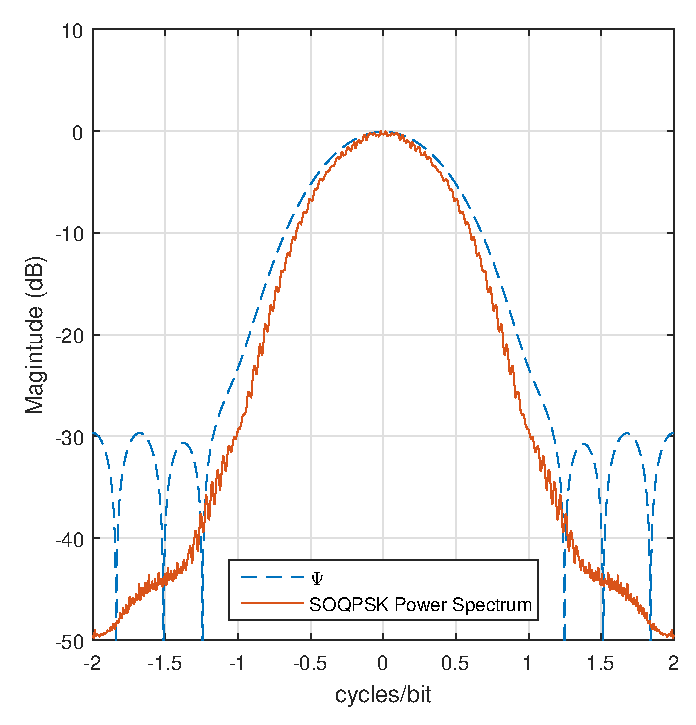
\includegraphics[width=5in]{figures/eq_equations/FDE2_spectrum_PSI.eps}
	\label{fig:SOQPSK_spectrum}
\end{figure}
